\section{Results}
\label{sec:3-results}
The results section will: 1. introduce the data instance from the case company;
2. show the effect of forcing work orders into specific weekly schedules $
\ElementPeriod \in \SetPeriod$; 3. show the effect of changing the  period
capacities $\ParStrategicResource$, and 4. show the effect of dynamically
changing the $\ParStrategicValue$ associated with $\ElementPeriod \in
\SetPeriod$ and $\ElementWorkOrder \in \SetWorkOrder$.

\subsection{Data Instance}
\begin{table}[H]
\centering
\begin{tabular}{|c|c|c|c|c|}
\hline
           & \begin{tabular}[c]{@{}c@{}}$|\SetWorkOrder{}|$\end{tabular} & \begin{tabular}[c]{@{}c@{}}$|\SetResource|$\end{tabular} & \begin{tabular}[c]{@{}c@{}}$|\SetPeriod|$\end{tabular} \\ \hline
Instance 1 & 3487                                                          & 16                                                               & 52                                                            \\ \hline
\end{tabular}

\caption{List of data instances from the case company. Here $\SetWorkOrder$ is the set of work orders, $\SetResource$ is the set of resources, and $\SetPeriod$ is the set of weekly periods.} % \label{fig1}
\end{table}

\subsection{Response to Inclusion}
The response to the inclusion of a work order is given by I parameter of the model which 
is constrained in \ref{eqn:constraint:strategic:include} of model given in .

The inclusion is made of forcing certain allocations of work orders to be in specific periods. Below a table is provided 
to show what changes will occur and at what and at what point in time.
\begin{table}[H]
	\centering
	\begin{tabular}{|c|c|c|c|c|c|}
	\hline
	\begin{tabular}[c]{@{}c@{}}\end{tabular}     & \begin{tabular}[c]{@{}c@{}}$\VarMetaTime_1 = 60$\end{tabular} & \begin{tabular}[c]{@{}c@{}} $\VarMetaTime_2 = 120$ \end{tabular} & \begin{tabular}[c]{@{}c@{}}$\VarMetaTime_3 = 180$\end{tabular} & \begin{tabular}[c]{@{}c@{}}$\VarMetaTime_4 = 240$\end{tabular} & \begin{tabular}[c]{@{}c@{}}$\VarMetaTime_5 = 300$\end{tabular} \\ \hline
	\begin{tabular}[c]{@{}c@{}}$\Delta |\SetPeriod|$\end{tabular} & 10                                                       & 20                                                       & 30                                                       & 40                                                       & 50                                                       \\ \hline
	\end{tabular}
\end{table}

With the inputs defined we will explain the main results which are shown in the figure below. 
\begin{figure}[H]
	\centering
	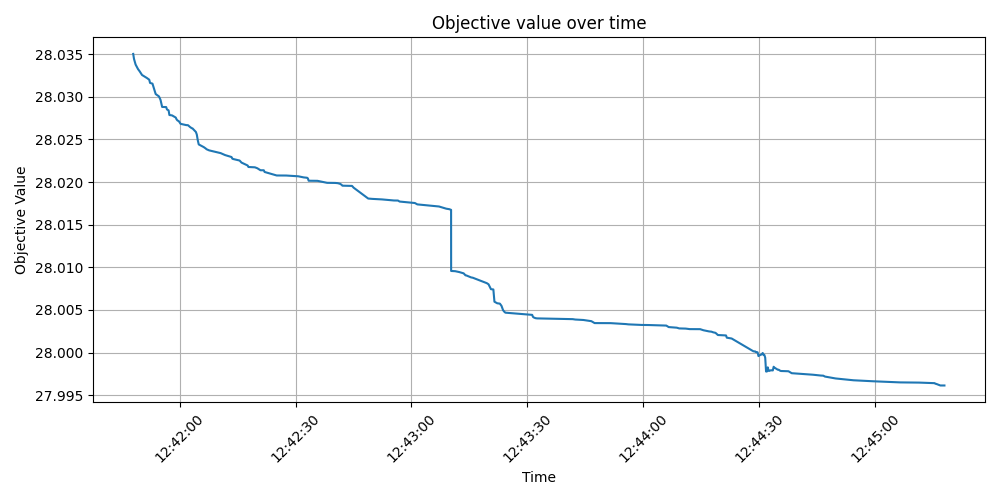
\includegraphics[width=1.0\textwidth]{figures/objective.png}
	\caption{Figure Caption}
	\label{fig:response-to-inclusion}
\end{figure}

\subsection{Response to Exclusion}
\begin{figure}[H]
	\centering
	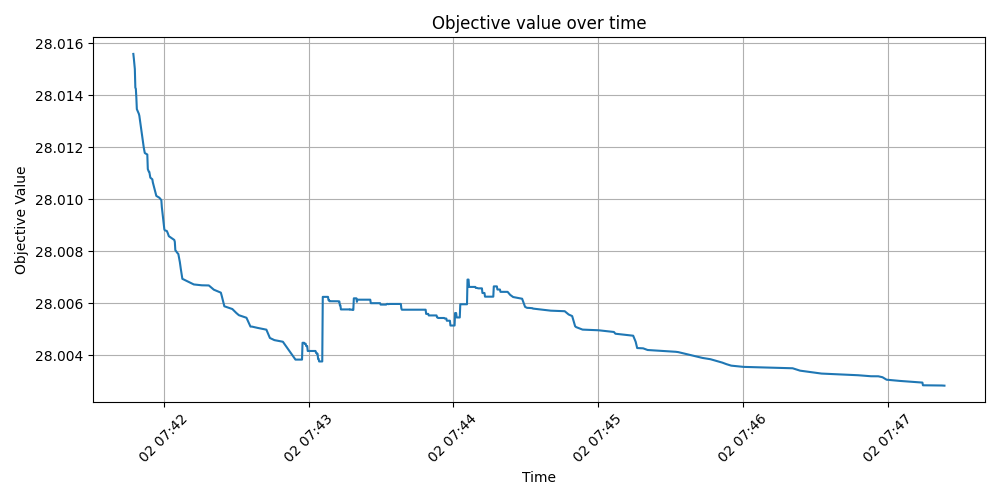
\includegraphics[width=1.0\textwidth]{figures/objective-400-exclusions.png}
	\caption{Figure Caption}
	\label{fig:objective-exclusion-400}
\end{figure}

\subsection{Response to Changes in Knapsack Capacities}
The effects of changes to capacities will be illustrated in the same way as it was with the response to inclusion and below we see the table that shows which inputs that the AbLNS will be affected by.

\begin{table}[H]
	\centering
	\begin{tabular}{|c|c|c|c|c|c|}
	\hline
	                      & \begin{tabular}[c]{@{}c@{}}$\VarMetaTime_1 = 60$\end{tabular} & \begin{tabular}[c]{@{}c@{}}$\VarMetaTime_2 = 120$\end{tabular} & \begin{tabular}[c]{@{}c@{}}$\VarMetaTime_3 = 180$\end{tabular} & \begin{tabular}[c]{@{}c@{}}$\VarMetaTime_4 = 240$\end{tabular} & \begin{tabular}[c]{@{}c@{}}$\VarMetaTime_5 = 300$\end{tabular} \\ \hline
	$\Delta |\SetPeriod|$ & 16                                                       & 16                                                       & 16                                                       & 16                                                       & 16                                                       \\ \hline
	$\Delta |\SetResource|$ & 16                                                       & 16                                                       & 16                                                       & 16                                                       & 16                                                       \\ \hline
	$\Delta |\ParStrategicResource|$& 100                                                      & 200                                                      & 400                                                      & 800                                                      & 1600                                                     \\ \hline
	\end{tabular}
\end{table}

\begin{figure}[H]%% placement specifier
	\centering
	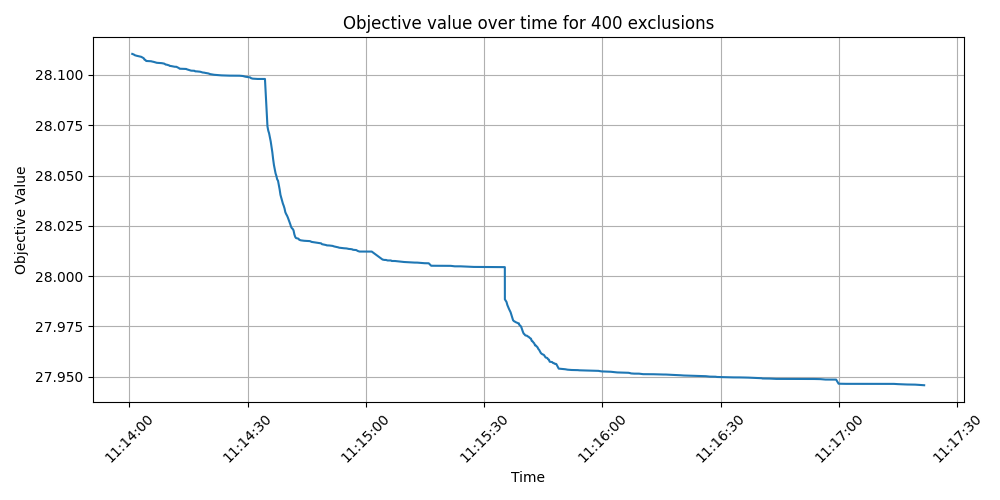
\includegraphics[width=1.0\textwidth]{figures/objective-resource-increases.png}
	\caption{Figure Caption}\label{fig:objective-resource-increases}
\end{figure}

Correspondingly we also have the figure below in which the resources are decreasing.

\subsection{Response to Changes in Item Weights}
The final parameter that will be changed is the work order value $\ParStrategicValue$. This section will be more elaborate as we have to show how that the
work orders are rearranged due to the changes in their value across the different periods.

\begin{table}[H]
	\centering
	\begin{tabular}{|c|c|c|c|c|c|}
	\hline
	             & \begin{tabular}[c]{@{}c@{}}$\VarMetaTime_1 = 60$\end{tabular} & \begin{tabular}[c]{@{}c@{}}$\VarMetaTime_2 = 120$\end{tabular} & \begin{tabular}[c]{@{}c@{}}$\VarMetaTime_3 = 180$\end{tabular} & \begin{tabular}[c]{@{}c@{}}$\VarMetaTime_4 = 240$\end{tabular} & \begin{tabular}[c]{@{}c@{}}$\VarMetaTime_5 = 300$\end{tabular} \\ \hline
	$\Delta |\SetWorkOrder[\VarMetaTime_{n}]{} \triangle \SetWorkOrder[\VarMetaTime_{n-1}]{}              |$         & 20                                                       & 40                                                       & 80                                                       & 160                                                      & 320                                                      \\ \hline
	$\Delta |\SetPeriod[\VarMetaTime_{n}]{} \triangle \SetPeriod[\VarMetaTime_{n-1}]{}                    |$         & 26                                                       & 26                                                       & 26                                                       & 26                                                       & 26                                                       \\ \hline
	\makecell{$\Delta |\ParStrategicValue[\VarMetaTime_{n}]| -$\\ $|\ParStrategicValue[\VarMetaTime_{n - 1}]|$}        & $1 \cdot 10^{5}$                                         & $2 \cdot 10^{5}$                                         & $4 \cdot 10^{5}$                                         & $8 \cdot 10^{5}$                                         & $1.6 \cdot 10^{6}$                                       \\ \hline
	\end{tabular}
\end{table}


\tikzpicture[gnuplot]
%% generated with GNUPLOT 6.0p1 (Lua 5.2; terminal rev. Jun 2020, script rev. 118)
%% Mon 25 Nov 2024 02:16:33 PM UTC
\path (0.000,0.000) rectangle (16.000,12.000);
\gpcolor{color=gp lt color border}
\gpsetlinetype{gp lt border}
\gpsetdashtype{gp dt solid}
\gpsetlinewidth{1.00}
\draw[gp path] (2.116,0.616)--(2.296,0.616);
\draw[gp path] (15.447,0.616)--(15.267,0.616);
\node[gp node right] at (1.932,0.616) {$1.9\times10^{11}$};
\draw[gp path] (2.116,2.462)--(2.296,2.462);
\draw[gp path] (15.447,2.462)--(15.267,2.462);
\node[gp node right] at (1.932,2.462) {$1.91\times10^{11}$};
\draw[gp path] (2.116,4.308)--(2.296,4.308);
\draw[gp path] (15.447,4.308)--(15.267,4.308);
\node[gp node right] at (1.932,4.308) {$1.92\times10^{11}$};
\draw[gp path] (2.116,6.154)--(2.296,6.154);
\draw[gp path] (15.447,6.154)--(15.267,6.154);
\node[gp node right] at (1.932,6.154) {$1.93\times10^{11}$};
\draw[gp path] (2.116,7.999)--(2.296,7.999);
\draw[gp path] (15.447,7.999)--(15.267,7.999);
\node[gp node right] at (1.932,7.999) {$1.94\times10^{11}$};
\draw[gp path] (2.116,9.845)--(2.296,9.845);
\draw[gp path] (15.447,9.845)--(15.267,9.845);
\node[gp node right] at (1.932,9.845) {$1.95\times10^{11}$};
\draw[gp path] (2.116,11.691)--(2.296,11.691);
\draw[gp path] (15.447,11.691)--(15.267,11.691);
\node[gp node right] at (1.932,11.691) {$1.96\times10^{11}$};
\draw[gp path] (2.116,0.616)--(2.116,0.796);
\draw[gp path] (2.116,11.691)--(2.116,11.511);
\node[gp node center] at (2.116,0.308) {$1.73254\times10^{9}$};
\draw[gp path] (3.449,0.616)--(3.449,0.796);
\draw[gp path] (3.449,11.691)--(3.449,11.511);
\node[gp node center] at (3.449,0.308) {$1.73254\times10^{9}$};
\draw[gp path] (4.782,0.616)--(4.782,0.796);
\draw[gp path] (4.782,11.691)--(4.782,11.511);
\node[gp node center] at (4.782,0.308) {$1.73254\times10^{9}$};
\draw[gp path] (6.115,0.616)--(6.115,0.796);
\draw[gp path] (6.115,11.691)--(6.115,11.511);
\node[gp node center] at (6.115,0.308) {$1.73254\times10^{9}$};
\draw[gp path] (7.448,0.616)--(7.448,0.796);
\draw[gp path] (7.448,11.691)--(7.448,11.511);
\node[gp node center] at (7.448,0.308) {$1.73254\times10^{9}$};
\draw[gp path] (8.782,0.616)--(8.782,0.796);
\draw[gp path] (8.782,11.691)--(8.782,11.511);
\node[gp node center] at (8.782,0.308) {$1.73254\times10^{9}$};
\draw[gp path] (10.115,0.616)--(10.115,0.796);
\draw[gp path] (10.115,11.691)--(10.115,11.511);
\node[gp node center] at (10.115,0.308) {$1.73254\times10^{9}$};
\draw[gp path] (11.448,0.616)--(11.448,0.796);
\draw[gp path] (11.448,11.691)--(11.448,11.511);
\node[gp node center] at (11.448,0.308) {$1.73254\times10^{9}$};
\draw[gp path] (12.781,0.616)--(12.781,0.796);
\draw[gp path] (12.781,11.691)--(12.781,11.511);
\node[gp node center] at (12.781,0.308) {$1.73254\times10^{9}$};
\draw[gp path] (14.114,0.616)--(14.114,0.796);
\draw[gp path] (14.114,11.691)--(14.114,11.511);
\node[gp node center] at (14.114,0.308) {$1.73254\times10^{9}$};
\draw[gp path] (15.447,0.616)--(15.447,0.796);
\draw[gp path] (15.447,11.691)--(15.447,11.511);
\node[gp node center] at (15.447,0.308) {$1.73254\times10^{9}$};
\draw[gp path] (2.116,11.691)--(2.116,0.616)--(15.447,0.616)--(15.447,11.691)--cycle;
\node[gp node right] at (13.979,11.357) {'<cat' using 1:2};
\gpcolor{rgb color={0.580,0.000,0.827}}
\draw[gp path] (14.163,11.357)--(15.079,11.357);
\draw[gp path] (3.382,10.823)--(3.382,10.692)--(3.449,10.690)--(3.449,10.463)--(3.449,10.279)%
  --(3.516,9.996)--(3.516,9.892)--(3.516,9.833)--(3.516,9.426)--(3.582,9.155)--(3.582,9.126)%
  --(3.582,9.045)--(3.582,8.885)--(3.649,8.569)--(3.649,8.299)--(3.716,8.293)--(3.716,8.237)%
  --(3.782,8.082)--(3.782,7.751)--(3.849,7.706)--(3.849,7.496)--(3.916,7.312)--(3.982,7.297)%
  --(3.982,7.195)--(4.049,7.029)--(4.049,6.953)--(4.116,6.942)--(4.116,6.868)--(4.116,6.861)%
  --(4.182,6.019)--(4.249,5.929)--(4.249,5.830)--(4.316,5.242)--(4.316,5.666)--(4.316,5.565)%
  --(4.382,4.878)--(4.449,5.513)--(4.449,4.890)--(4.516,4.887)--(4.516,4.396)--(4.516,4.845)%
  --(4.582,4.847)--(4.649,4.727)--(4.649,4.486)--(4.649,4.649)--(4.716,4.635)--(4.716,3.837)%
  --(4.782,4.107)--(4.782,4.152)--(4.782,3.991)--(4.849,3.804)--(4.849,4.008)--(4.916,3.846)%
  --(4.982,4.173)--(4.982,4.146)--(4.982,4.186)--(5.049,3.894)--(5.115,4.145)--(5.115,3.989)%
  --(5.115,3.715)--(5.249,4.077)--(5.249,3.594)--(5.249,3.988)--(5.315,3.719)--(5.315,3.960)%
  --(5.382,3.791)--(5.382,3.656)--(5.449,3.643)--(5.449,3.342)--(5.515,3.394)--(5.515,3.423)%
  --(5.582,3.255)--(5.649,3.024)--(5.715,3.386)--(5.782,3.157)--(5.782,3.195)--(5.782,3.324)%
  --(5.849,3.138)--(5.849,3.287)--(5.915,2.788)--(5.915,2.581)--(5.915,2.710)--(5.982,2.375)%
  --(5.982,2.189)--(6.049,2.611)--(6.115,2.189)--(6.182,2.000)--(6.182,2.319)--(6.182,2.289)%
  --(6.249,2.371)--(6.249,1.744)--(6.249,2.251)--(6.315,2.162)--(6.315,2.050)--(6.382,2.185)%
  --(6.382,1.717)--(6.382,1.868)--(6.449,1.466)--(6.515,1.903)--(6.582,1.886)--(6.582,1.740)%
  --(6.649,1.748)--(6.649,1.850)--(6.715,1.868)--(6.782,1.469)--(6.782,1.831)--(6.782,1.800)%
  --(6.849,1.639)--(6.849,1.839)--(6.849,2.490)--(6.915,2.258)--(6.915,2.517)--(6.982,2.418)%
  --(6.982,2.318)--(6.982,2.369)--(7.048,2.366)--(7.048,1.919)--(7.115,2.095)--(7.115,2.183)%
  --(7.182,2.227)--(7.182,1.578)--(7.248,2.004)--(7.315,1.780)--(7.315,2.238)--(7.382,1.872)%
  --(7.382,1.941)--(7.448,2.161)--(7.515,2.051)--(7.515,2.151)--(7.582,2.141)--(7.648,2.129)%
  --(7.715,2.086)--(7.715,1.969)--(7.782,2.150)--(7.782,2.087)--(7.782,2.153)--(7.848,2.020)%
  --(7.848,1.754)--(7.915,1.999)--(7.915,1.990)--(7.915,1.900)--(7.982,1.994)--(8.048,1.983)%
  --(8.048,2.049)--(8.048,2.174)--(8.115,2.030)--(8.115,1.768)--(8.182,1.903)--(8.182,1.857)%
  --(8.248,1.738)--(8.248,1.850)--(8.315,2.019)--(8.382,1.970)--(8.382,1.843)--(8.448,2.003)%
  --(8.448,1.818)--(8.515,2.046)--(8.515,1.663)--(8.515,1.955)--(8.582,2.153)--(8.582,2.169)%
  --(8.648,1.907)--(8.648,2.096)--(8.648,2.148)--(8.715,2.093)--(8.782,1.821)--(8.782,2.113)%
  --(8.848,2.052)--(8.848,1.448)--(8.915,1.964)--(8.981,1.977)--(8.981,1.992)--(9.048,1.787)%
  --(9.048,1.333)--(9.048,1.960)--(9.115,1.392)--(9.115,1.254)--(9.181,1.765)--(9.181,1.694)%
  --(9.248,1.803)--(9.248,1.823)--(9.315,1.627)--(9.315,1.532)--(9.315,1.756)--(9.381,1.242)%
  --(9.448,1.599)--(9.448,1.860)--(9.448,1.751)--(9.515,1.616)--(9.581,1.690)--(9.581,1.731)%
  --(9.648,1.809)--(9.648,1.611)--(9.648,1.639)--(9.781,1.503)--(9.781,1.834)--(9.781,1.720)%
  --(9.848,1.619)--(9.848,1.697)--(9.848,1.673)--(9.915,1.607)--(9.915,1.513)--(9.915,1.415)%
  --(9.981,1.596)--(9.981,1.497)--(10.048,1.301)--(10.048,1.358)--(10.115,1.481)--(10.181,1.440)%
  --(10.248,1.319)--(10.248,1.262)--(10.315,1.336)--(10.315,1.613)--(10.315,1.636)--(10.381,1.749)%
  --(10.381,1.553)--(10.448,1.812)--(10.448,1.297)--(10.448,1.557)--(10.515,1.441)--(10.515,1.642)%
  --(10.581,1.646)--(10.581,1.457)--(10.648,1.735)--(10.648,1.556)--(10.714,1.767)--(10.714,1.518)%
  --(10.781,1.480)--(10.781,1.692)--(10.848,1.666)--(10.848,1.531)--(11.048,1.370)--(11.114,1.519)%
  --(11.114,1.243)--(11.114,1.813)--(11.181,1.079)--(11.248,1.819)--(11.248,1.732)--(11.248,1.327)%
  --(11.314,1.335)--(11.381,1.731)--(11.381,1.768)--(11.381,1.855)--(11.448,1.739)--(11.448,1.204)%
  --(11.448,1.506)--(11.514,1.805)--(11.581,1.809)--(11.581,1.874)--(11.648,1.813)--(11.714,1.609)%
  --(11.714,1.813)--(11.781,1.812)--(11.848,1.573)--(11.848,1.844)--(11.848,1.459)--(11.914,1.368)%
  --(11.914,1.436)--(11.914,1.606)--(11.981,1.736)--(12.048,1.681)--(12.048,1.703)--(12.114,1.662)%
  --(12.181,1.677)--(12.181,1.835)--(12.248,1.833)--(12.248,1.673)--(12.314,1.651)--(12.314,1.449)%
  --(12.381,1.734)--(12.381,1.744)--(12.381,1.430)--(12.448,1.745)--(12.448,1.627)--(12.514,1.612)%
  --(12.514,1.431)--(12.581,1.568)--(12.581,1.237)--(12.647,1.554)--(12.647,1.581)--(12.714,1.537)%
  --(12.714,1.429)--(12.847,1.736)--(12.847,1.463)--(12.914,1.585)--(12.981,1.524)--(12.981,1.697)%
  --(13.047,1.800)--(13.114,1.514)--(13.114,1.612)--(13.181,1.830)--(13.181,1.621)--(13.247,1.639)%
  --(13.314,1.534)--(13.314,1.606)--(13.314,1.721)--(13.381,1.751)--(13.447,1.775)--(13.447,1.803)%
  --(13.514,1.818)--(13.514,1.781)--(13.581,1.713)--(13.581,1.479)--(13.581,1.376)--(13.647,1.731)%
  --(13.647,1.643)--(13.714,1.779)--(13.781,1.384)--(13.781,1.754)--(13.847,1.836)--(13.847,1.687)%
  --(13.914,1.724)--(13.914,1.607)--(13.981,1.393)--(13.981,1.113)--(13.981,1.688)--(14.047,1.409)%
  --(14.114,1.653)--(14.114,1.539)--(14.181,1.226)--(14.181,1.647)--(14.181,1.585)--(14.314,1.657)%
  --(14.314,1.691)--(14.314,1.531)--(14.381,1.569)--(14.381,1.695)--(14.447,1.464)--(14.447,1.668)%
  --(14.514,1.497)--(14.580,1.158)--(14.580,1.462)--(14.580,1.690)--(14.647,1.718)--(14.780,1.825)%
  --(14.780,1.583)--(14.847,1.843)--(14.914,1.888)--(14.980,1.631)--(14.980,1.991)--(14.980,1.640)%
  --(15.047,1.828)--(15.047,1.867)--(15.114,1.538)--(15.114,1.941)--(15.180,1.965)--(15.247,1.853)%
  --(15.247,1.984)--(15.314,2.064)--(15.380,1.936)--(15.380,1.829);
\gpcolor{color=gp lt color border}
\draw[gp path] (2.116,11.691)--(2.116,0.616)--(15.447,0.616)--(15.447,11.691)--cycle;
%% coordinates of the plot area
\gpdefrectangularnode{gp plot 1}{\pgfpoint{2.116cm}{0.616cm}}{\pgfpoint{15.447cm}{11.691cm}}
\endtikzpicture
%% gnuplot variables

